
\documentclass[letterpaper,twocolumn,10pt]{article}
\usepackage{usenix,epsfig,endnotes}
\usepackage{amsmath}
\usepackage[noend]{algpseudocode}
\usepackage{paralist,algorithm}
\usepackage{booktabs}
\usepackage{subcaption}
\usepackage{multirow}
\usepackage{float}
\usepackage{graphicx}
\usepackage{pgfplots}
\usepackage{amssymb}
\usepackage{epstopdf}
\usepackage{tikz}
\usepackage{tkz-tab}
\usepackage{titlesec}
\usepackage{xspace}
%\usepackage{epsfig}
%\epstopdfsetup{outdir=./}
%\usepackage[showframe=true]{geometry}
\usepackage{enumitem}
\usepackage{adjustbox}

\addtolength{\columnsep}{-1mm}
\addtolength{\belowcaptionskip}{-1pt}
\setlength{\parskip}{3pt}
\setlength{\textfloatsep}{5pt}
\topmargin=1pt
\topskip=1pt


\titlespacing*{\section}
{2pt}{2pt}{2pt}
\titlespacing*{\subsection}
{2pt}{2pt}{2pt}
\titlespacing*{\subsubsection}
{2pt}{2pt}{2pt}

\titlespacing{\section}
{2pt}{2pt}{2pt}
\titlespacing{\subsection}
{2pt}{2pt}{2pt}
\titlespacing{\subsubsection}
{2pt}{2pt}{2pt}


\begin{document}

\title{Setting budgets for live debugging}

\iffalse
\author{
{\rm Nipun Arora$^\dagger$, Franjo Ivan\v{c}i\'{c}}\\$^*$, Gail Kaiser$^\ddagger$}\\
$^\dagger$NEC Laboratories America \hspace{1.4cm}   $^\*$Google NYC \hspace{1.4cm}  $^\ddagger$Columbia University\\
nipun@nec-labs.com \hspace{4pt} ivancic@google.com \hspace{4pt} kaiser@cs.columbia.edu \\
}
\fi

%\iffalse
\author{
{\rm Nipun Arora}\\
       NEC Research Labs\\
       Princeton, NJ, USA\\
       nipun@nec-labs.com
\and
{\rm Franjo Ivan\v{c}i\'{c}}\\
       Google\\
       New York, NY, USA\\
       ivancic@google.com
\and
{\rm Gail Kaiser}\\
       Columbia University\\
       New York, NY, USA\\
       kaiser@cs.columbia.edu
}
%\fi
\maketitle


\newcommand{\iprobe}{\texttt{iProbe}\xspace}
\newcommand{\parikshan}{\texttt{Parikshan}\xspace}
\newcommand{\comment}[1]{}
\newtheorem{example}{Example}
\def\infinity{\rotatebox{90}{8}}


%SIGMETRICS
\begin{abstract}
\noindent
One of the biggest problems faced by developers debugging large scale systems is replicating the deployed environment to figure out errors. 
Additionally, many modern companies are combining their development and operation management activities (DevOps), which has led to an increased emphasis on fast bug resolution. 
In this work we present \textit{``live-debugging''}, a mechanism which allows debugging a production system (run test-cases, debug, or profile, etc.) on-the-fly. 
%in a sandbox environment cloned from the live running system. 
The paper leverages user-space containers (OpenVZ/LXC) to launch containers cloned and migrated from running instances of an application, thereby launching two containers: \textit{production} (which provides the real output), and \textit{debug-container} (for debugging). 
This \emph{debug-container} provides a sandbox environment for debugging without any perturbation to the execution environment. 
%Our sandboxes provide name-space, and resource management for the processes executing the test/debug cases. 
Customized network-proxy agents replicate or replay network inputs from clients to both the production and debug-container, as well as safely discard all network output from the debug-container. 
The sandboxed debug-container can be run either on the same physical host as the production container, or scaled out on dedicated physical debug servers. 
We used our system, called \texttt{Parikshan}, to do \textit{``live-debugging''} on several real-world bugs, and effectively reduced debugging complexity and time.
%We believe our tool provides a mechanism for practical live-debugging of large scale multi-tier and cloud applications, without requiring any application down-time, and minimal performance impact.

\noindent
\textbf{Tags:} live cloning, network duplication, live debugging
\end{abstract}

%In recent years there has been a lot of work in record-and-replay systems which captures traces from live production systems, and replays them.
%However, most such record-replay systems have a high recording overhead and are still not practical to be used in production environments without paying a penalty in terms of user-experience. 

\section{Introduction}
\label{sec:introduction}

Software bugs are \emph{everywhere}.
They often escape extermination efforts in software testing causing frustration to operators, and a loss of business revenue.
\emph{Bug Diagnosis} is the ``art'' of identifying the root-cause and the possible ``fix'' for the failure.
In general the process involves a trial-and-error process in the development environment. 
The debugger uses the input causing the failure and tries to localize the problem in a small part of the application.
He then manually skims through the code in the localized area to correctly identify the problem.
This process can be long and arduous, causing significant loss of revenue.

We believe that by closing the gap between the production and debugging environment, we can provide the developer with a deeper insight of the cause of the bug.
Our previously proposed approach called \livedebugging~\cite{livedebugging}, we have developed a framework which allows debuggers to safely debug applications within the production environment.
This is done by creating a parallel debugging environment, which gets the same input as the normal production system.
This debugging environment provides a powerful tool for the debugger, to freely instrument or modify the application without impacting the performance of the production system.

In this work, we focus on real-time debugging techniques, which can be used on the production environment.
Firstly, we will present an adaptive guided profiling mechanism, which can provide rich profiles in order to localize the bug, while keeping the instrumentation overhead within a preset limit(called budget).
We are inspired by previous approaches in delta debugging~\cite{delta}, and statistical debugging~\cite{statistical, holmes}. 
These approaches use sampled profiles from predetermined instrumentation points, and compare traces, with and without the bug, to localize the problem.
Holmes~\cite{holmes} in particular also includes a feedback loop, which iteratively modifies the instrumentation profiles to gather more relevant traces.
We use a similar technique along with dynamic instrumentation to iteratively change profiles to get a better understanding of the root-cause of the error while debugging the application on-the-fly.
Budgeting the overhead is important so that the instrumentation in the debug environment does not make it lag too far behind the production environment.

Secondly, we will also look at a more proactive approach, where we modify the debug container to not simply trace, but see if a potential fix/optimization solves the problem.
We show how for some performance bugs, we can dynamically patch and verify that the problem is indeed solved.

\section{Overview}
\label{sec:overview}


In recent years several monitoring techniques have been developed to monitor the health of production systems.
For example most modern operating systems have resource monitors~\cite{linuxHealth, windowsHealth, macHealth}, which can be used to track the CPU, memory usage, cache misses, temperature etc. of the physical machine.
These are useful to discover high workloads, or if the machine is stressed because of heavy resource usage.
Similarly, application level monitoring tools are used to report transactions or errors in the application.
Monitoring outputs usually provide the first clue towards resolving an error in the debugging process.
%While useful, these monitoring mechanisms  have a performance trade-off with the amount of instrumentation that can be done.
%Furthermore, the information provided by these logs may not be enough to understand the root-cause of the error.

However all monitoring/instrumentation techniques impose a performance overhead on the applications.
This can adversely impact user-experience, hence real-world production instrumentation is generally kept at very low levels.
\parikshan provides an alternative mechanism where this debugging/instrumentation can be done in parallel on a sandboxed cloned container.
Any instrumentation or monitoring in the debug-container has no performance impact on the production container.
In the context of our system, debuggers can use a variety of ad-hoc approaches to capture the root-cause of an error.
For example a naive approach could be to use trial-and-error instrumentation to find the execution trace for the error.
Alternatively, the user could also do aggressive brute force instrumentation for all function execution, which could help locate the problem.
However, both these approaches can have potentially high overheads, which in turn can lead to a buffer overflow.

In this chapter we introduce a statistical sampling approach which imposes a bounded performance overhead, to ensure maximal live debugging information, without causing a buffer overflow.
%In our search for more systematic approach towards live debugging, we looked towards two possible techniques.
%Firstly, we try to implement an automated budget limited instrumentation approach for capturing application logs.
We are inspired by previous work done in statistical debugging~\cite{cbi}, and delta debugging~\cite{delta} techniques which aim to streamline and automate the process of bug localization.
This is achieved by having predicate profiles from both successful and failing runs of a program and applying statistical techniques to pinpoint the cause of the failure.
The core advantage of statistical debugging is that the sampling frequency of the instrumentation can be decreased to reduce the instrumentation overhead.

One of the key criteria for successful statistical debugging is to have higher instrumentation rates, to make the results more statistically significant. 
There is a clear trade-off between instrumentation vs performance overhead for statistical instrumentation. 
A key advantage of using this with \parikshan is that we can provide live feedback based buffer size and bounded overheads, hence squeezing the maximum advantage out of statistical debugging without impacting the overhead. 
We evaluate the slack available in each request for instrumentation without risking a buffer overflow and getting out of sync of the production container.
Live interactive debugging provided by \parikshan further allows for quick updates to the instrumentation and targeting specific areas of the application code.


\begin{figure*}[ht!]
	\begin{center}
		%    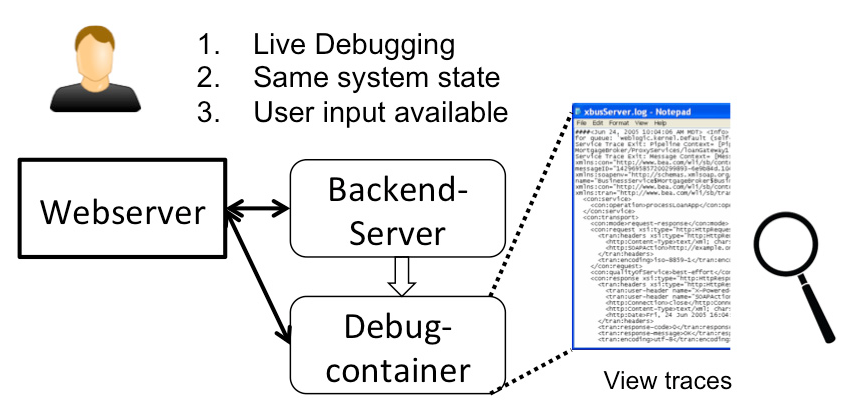
\includegraphics[width=0.7\textwidth]{figs/motivation.eps}
		\includegraphics[width=0.9\textwidth]{figs/workflow3.pdf}
		\caption{Workflow of \parikshan in a live multi-tier production system with several interacting services. When the administrator of the system observes errors in two of it's tiers, he can create a sandboxed clone of these tiers and observe/debug them in a sandbox environment without impacting the actual production system.}
		\label{fig:motivation}
	\end{center}
\end{figure*}


\section{Background}
\label{sec:background}

Before presenting our approach let us review basic concepts and terminology used in previous work in statistical/sampling based debugging approaches, and generating interesting predicates for capturing bugs.

\subsection{Terminology}
\label{sec: terminology-guided}


% ---- NIPUN -> THIS HAS BEEN COPIED IN PARTS FROM HOLMES BACKGROUND

The decision of what to monitor is crucial as the debugger can only decipher where the bug is located based on clues he  finds in the instrumentation output.
The decision of what to chose as an instrumentation point has been well studied in previous approaches \cite{}.
An \emph{instrumentation site} is a single program location at which the state of the running program will be inspected.
Instrumentation points are selected based on importance of the code location being tracked.
The idea behind instrumentation is to capture enough data to get a decent clue towards finding the bug.

Each of these instrumentation sites are decomposed into predicates which are conditionals with a true/false value.
Predicates can be branch conditionals, loops, function calls, return instructions and if conditionals.
Predicates provide significant advantages in terms of memory/performance overheads.
Instead of printing predicates, they are usually counted, and a profile is generated.
This reduces the amount of instrumentation overhead, and several predicates can easily be encoded in a small memory space.

Existing approaches also offer sampling as a means to more effective predicate instrumentation with minimal overhead.
This technique, creates instrumentation that yields a sparse but fair random subset of the complete counts.
Other approaches have extended this technique to adaptive automated sampling to better manage the overhead.

\subsection{Statistical Debugging}
\label{sec:Statistical Debugging}

% ---- NIPUN -> THIS HAS BEEN COPIED IN PARTS FROM HOLMES BACKGROUND

The Cooperative Bug Isolation Project forms the basis of our statistical debugging approach.
This project uses predicates at instrumentation points such as branch conditionals, call instructions etc., and statistically samples their counts to get a profile of the bug.
Each run of the program is further tagged with a feedback report for a single execution is a bit-vector with two bits for every path: one bit indicates whether the predicate was \emph{observed} and the other bit that indicates whether the predicate was executed in that run.
Predictors are scored based on \emph{sensitivity} (accounts for many failed runs) and \emph{specificity} (does not mis-predict failure in a successful run).
These scores are balanced using a numeric importance score computed as follows
The events corresponding to a predicate p from all the runs can be aggregated into four values: (1) $S_{o}(p)$: the number of successful runs in which the predicate p was observed (2) $F_{o}(p)$: the number of failed runs in which the predicate  p was observed (3) $S_{e}(p)$: the number of successful runs in which the predicate p was executed, and (4) $F_{e}(p)$: the number of failed runs in which the predicate p was executed.
Using these values, three scores of bug relevance are calculated.

\begin{equation}
\label{eq:sensitivity}
Sensitivity(p) = \frac{log|F_{e}(p)|}{log|F|}
\end{equation}

\begin{equation}
\label{eq:context}
Context(p) = \frac{F_{o}(p)}{S_{o}(p) + F_{o}(p)}
\end{equation}

\begin{equation}
\label{eq:increase}
Increase(p) = \frac{F_{e}(p)}{S_{e}(p) + F_{e}(p)} - Context(p)
\end{equation}

where F is the total number of failing runs. The harmonic mean of Sensitivity and Increase identifies predicates that are both highly sensitive and highly specific :

\begin{equation}
\label{eq:importance}
Importance = \frac{2}{\frac{1}{Sensitivity(p)}+\frac{1}{Increase(p)}}
\end{equation}

The Importance score is calculated for each path, and the top results are selected and presented to the programmer as potential root causes.

Nainar et Al\cite{}, further extend this approach in their work on adaptive statistical bug isolation.
They aim to reduce the instrumentation amount by initially instrumenting only a small part of the total predicates, then adaptively turn on the predicates which are more indicative of the error.
In particular, they define a vicinity function by which they aim to find predicates which are likely indicators of the error.
The main hypothesis is that predicates in the vicinity of existing predicates which are good error indicators, are also likely to be error indicators.

In the next section, we give a short description of the design of live debugging and our \parikshan framework to facilitate the exposition of the ideas in this paper. 
%A detailed explanation of the complete design of the paper can be found in ~\cite{parikshan}.

\subsection{The case for Live Debugging}
\label{sec:case}

Figure \ref{fig:motivation}, shows a high level overview of ``live debugging'' in action. 
The figure shows a live production system with multiple services. 
The system is maintained by an operator, who can observe the health of the system using light-weight monitoring, which is part of the deployed system. 
In the interest of application performance, production system monitoring is usually limited to system resource usage, application usage statistics, transaction logs, and error logs.

Let us assume that at a certain time in the execution of the system, the operator observes unusual memory usage in the glassfish application server, and some error logs being generated in the nginx webserver. 
Typically, trouble tickets are generated for such problems, and they are debugged offline.
However, the operator can now use \parikshan to fork off clones of the nginx and glassfish containers as \textbf{nginx-debug} and \textbf{glassfish-debug}.
Network duplication mechanisms ensure that the debug-containers receive the same inputs as the production, and the production containers continue to provide service without interruption.
This seperation of production and debug environments allows the operator to use dynamic instrumentation tools to do deeper diagnosis without fearing any problems in the user-facing operations.
Since the system has been cloned from the original potentially ``buggy'' production container, it will also exhibit the same memory leaks/or logical errors.
Additionally, \parikshan can focus on the ``buggy'' parts of the system, without needing to replicate the entire system in a test-cluster. 
This process will greatly reduce the time to bug resolution, and allow real-time bug diagnosis capability.

\subsubsection{Design Overiview}
\label{sec:designBackground}

Our system called \parikshan, is composed of three modules: 

%\begin{itemize}
%	\item 

 \textbf{Clone Manager}: manages ``live cloning'' between the production and debug containers.
``Live Cloning'' refers to the process of copying a running virtual machine, or container from one server to another, without disconnecting any client or process running within the service.
This generates two containers, a production container which serves the actual user requests, and a debug-container which gets the same input as the production but is maintained only for debugging purposes.
The ``live'' part in the cloning process means that cloning has a very small suspend time and the service is kept active while cloning. \\

\iffalse	
	\begin{figure}[ht]
		\begin{centering}
			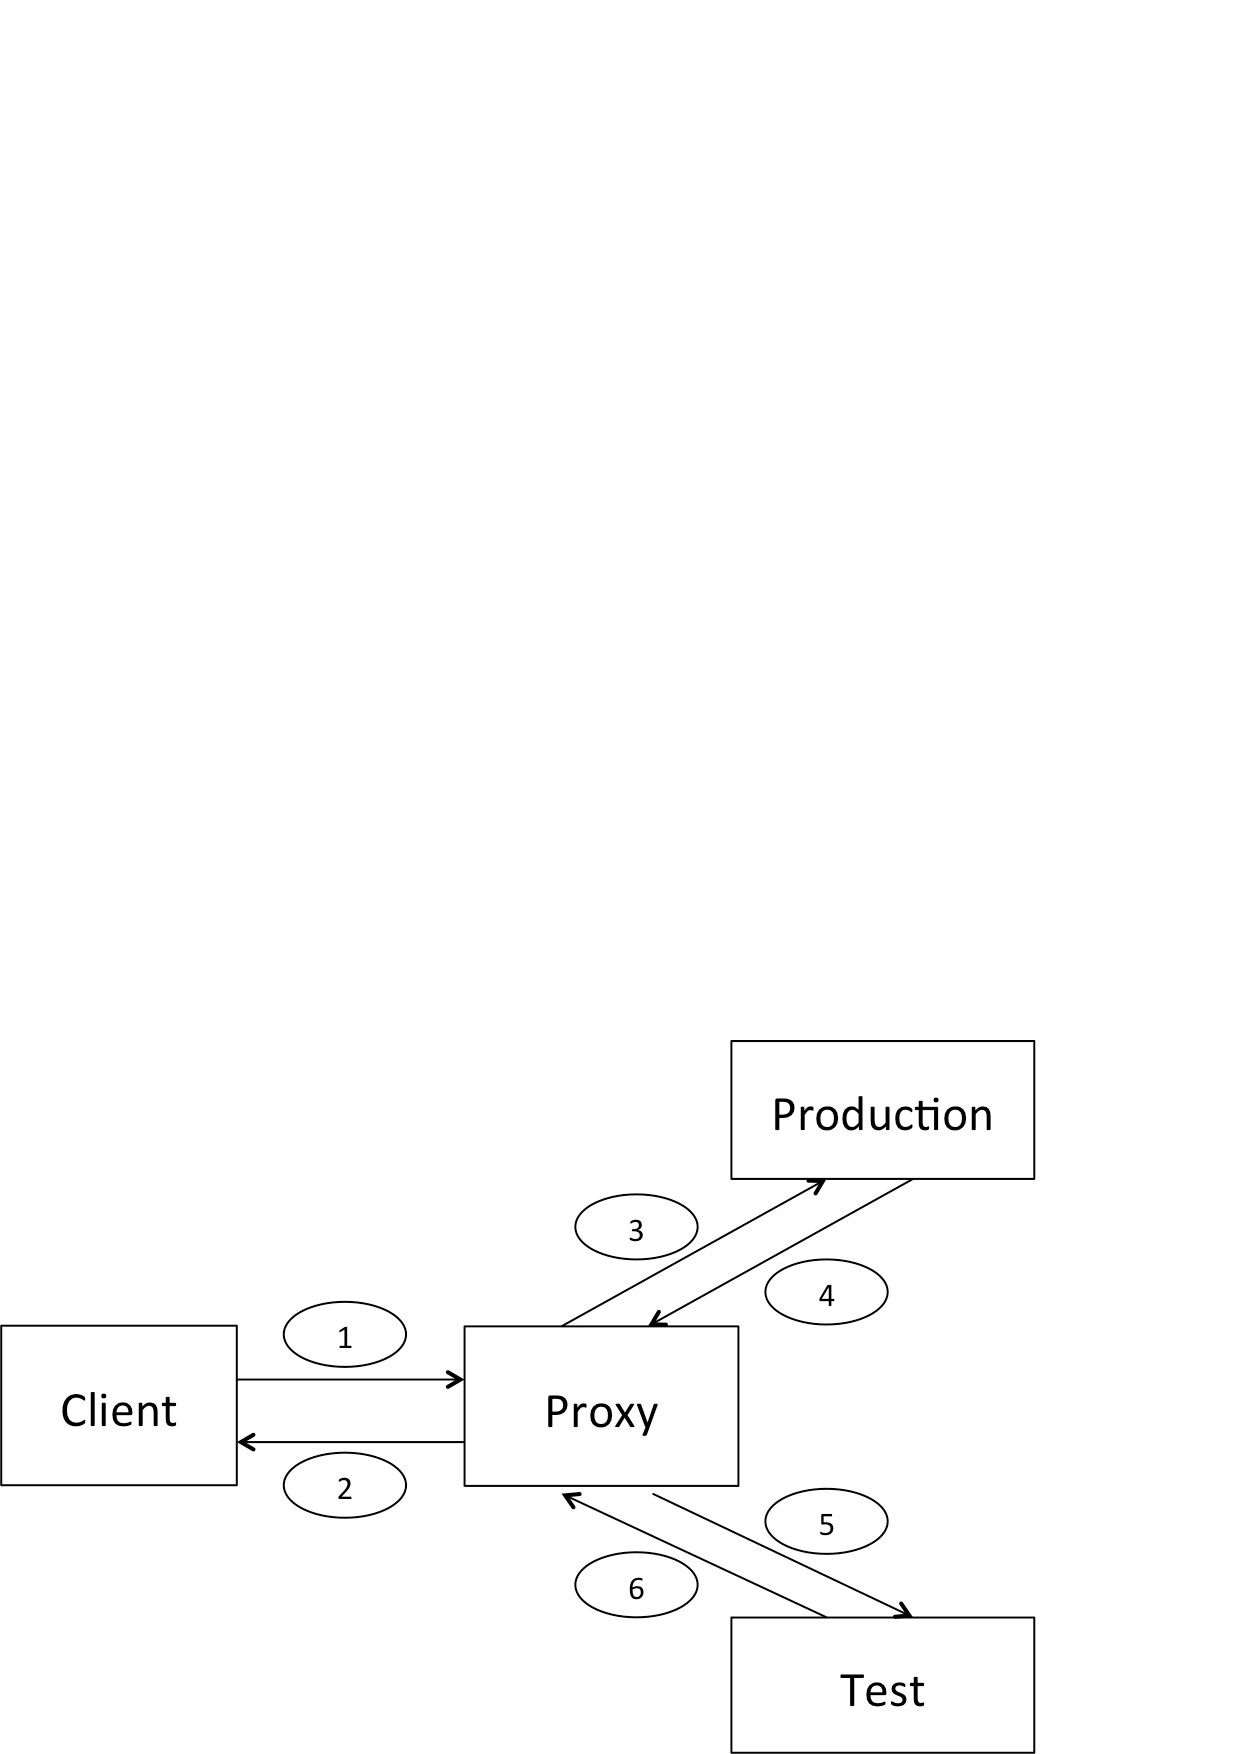
\includegraphics[width=0.4\textwidth]{figs/network_dup.pdf}
			%    \captionsetup{justification=centering}
			\caption{Description of the Network Duplicator. In \textit{synchronized} mode: Thread 1 executes steps [1,3,5], and Thread 2 executes [2,4,6] sequentially. In \textit{asynchronous} mode: Thread 1 executes steps [1,3], Thread 2 executes [2,4], Thread 3 executes [5], and Thread 4 executes [6]}
			\label{fig:duplicator}
		\end{centering}
	\end{figure}
\fi
%\item 
 \textbf{Network Duplicator}: The network duplicator manages communication from the client to both the production container and the debug container.
The basic design is based on a customized TCP level proxy, which duplicates network traffic to both these containers.
As shown in figure~\ref{fig:duplicator}, the duplicator uses an asynchronous packet forwarding model, with 4 threads for each incoming connections.
Thread T1 forwards packets from client to proxy (link 1), and from proxy to production container(link 2). It then uses a non-blocking send to foward packets to an internal pipe buffer shared between thread T1, thread T3. Thread T3, then reads from this piped buffer and sends traffic forward to the debug-container. 
Similarly Thread T2, receives packets from production container, and forwards them to the client, while thread T4, receives packets from debug container and drop them. 

The advantage of this strategy is that any slowdown in the debug-container will not impact the production container.
However, a side-effect is that if the speed of the debug-container is too slow compared to the production container, it may lead to a buffer overflow. 
We call the time taken by a connection before it overflows, it's \textbf{debugging window}.
We assume that both the production and debug containers are identical for the purposes of debugging as long as we do not have an overflow. \\

\textbf{Network Aggregator}: The network aggregator manages communication from 
	
%\end{itemize}

\section{Problem Formulation}
\label{sec:model}

As explained in section~\ref{sec:design}, the asynchronous packet forwarding in our network duplication results in a ``debug window''. 
The ``debug window'' is the time before the buffer of the debug-container overflows because of the input from the user. 
The TCP connection from end-users to production-containers are synchronized by default.
This means that that the rate of incoming packets is limited by the amount of packets that can be processed by the production container. 
On the other hand, packets are forwarded asynchronously to an internal-buffer in the debug-container.
The duration of the ``debug window'' is dependent on the incoming workload, the size of the buffer, and the overhead/slowdown caused due to instrumentation in the debug-container.

In this section we try to model the testing window by using concepts well used in queuing theory(for the sake of brevity we will avoid going into too much detail, readers can find more about queuing theory models in~\cite{queueWiki}).
The buffer overflow of our test-container can be modeled as a M/M/1/K queue (Kendall's notation~\cite{kendall}), for our simplest asynchronous model, and as a M/M/c/K queue in the asynchronous load-balanced model.
An M/M/1/K queue, denotes a queue where requests arrive according to a poisson process with rate $\lambda$, that is the inter-arrival times are independent, exponentially distributed random variables with parameter $\lambda$ . 
The service times are also assumed to be independent and exponentially distributed with parameter $\mu$. Furthermore, all the involved random variables are supposed to be independent of each other. 
Further, the notation specifies that there are $c$ queues/ or alternatively $c$ servers managing the requests, and the queues is of a finite capacity, i.e. the queue can accommodate a maximum of K requests.
In our case $\lambda$ denotes the rate at which requests arrive to the buffer from the production container, and $\mu$ denotes the processing time overhead of each request in the test-container (to simplify the problem, we ignore the actual processing time of the test-container, as the incoming rate $\lambda$ is already synchronized with the production container processing time, and it is only the overhead added by the test-container which matters). 
In our simple asynchronous forwarding strategy, we have $c=1$ as we have only a single test-container, potentially as explained earlier, in a load-balanced asynchronous model this could be extended to $c$ servers to increase the time window.

Now based on this notation the expected size of the time window is :

\section{Related Work}
\label{sec:related}

Queuing theory has been used to solve several real-world problems. 
In particular queuing theory has found uses in supply chain optimization.
For example Fedex, and retailers like best-buy have used queuing theory to optimize their delivery schedules.
In the IT field, it has been used by companies like youtube, to optimize queuing in various transaction oriented service systems.
Similarly several other transaction based service oriented applications, are often used for optimizing, and providing service level agreement guarantees.

One other area, where queuing theory has been frequently applied is for load balancing service applications.
For example a common use-case is traffic being routed from a DNS server to numerous webservers. 
Depending on the traffic load the DNS server acts like a proxy and forwards traffic to the webserver, which is relatively free (round robin scheme, or first in first out etc.).
Queuing theory can help model such traffic forwarding, by suggesting more scaled out system depending on the workload, and the amount of accepted transaction processing time.
In this paper we have extended a similar model towards our proxy buffer capacity modeling and instrumentation, in order to extend the time-window to it's maximum.
\section{Conclusion and Future Work}
\label{sec:conclusion}

In conclusion we say something something..

\bibliographystyle{abbrv}
\bibliography{sigproc}  % sigproc.bib is the name of the Bibliography in this case
% You must have a proper ".bib" file
%  and remember to run:
% latex bibtex latex latex
% to resolve all references
\end{document}
